\documentclass{article}
\usepackage[utf8]{inputenc}
\usepackage{amsmath}
\usepackage{amsthm}
\usepackage{amssymb}
\usepackage{dsfont}
\usepackage[margin=1.5in]{geometry}
\usepackage{mathtools}
\usepackage{cancel}
\usepackage{xfrac}
\usepackage{siunitx} % for scientific notation \num{}
\usepackage{authblk} % for authors
\usepackage{tikz} % for circled{}
\usepackage{systeme} % for system of equations bracket
\usepackage{verbatim} % for comment
\usepackage{xfp} % for floating point operations in macros
\usepackage{graphicx} % for cropping the images
\usepackage{subcaption}
\usepackage{dsfont} % for doublestroke fonts
\usepackage{float}
\usepackage[colorlinks=true,citecolor=blue]{hyperref} % hyperlink
\usepackage[scr=rsfso,frak=euler,bb=ams]{mathalfa} % math letters
\usepackage[english]{babel}
\usepackage[square,numbers]{natbib}
\usepackage[nottoc,numbib]{tocbibind}
\usepackage{xparse}
\bibliographystyle{abbrvnat}

\makeatletter
\newcommand*{\toccontents}{\@starttoc{toc}}
\makeatother

\begin{document}

\begin{center}
    \Large Quadcopter Dynamics and Numerical Simulation \\
    \large MAE 542 Final Project \\
    \vspace{0.5em}
    \small Matthew Coleman \\
    \small December 6, 2022
\end{center}

\toccontents

\newpage
\section{Introduction}

\begin{figure}[H]
    \centering
    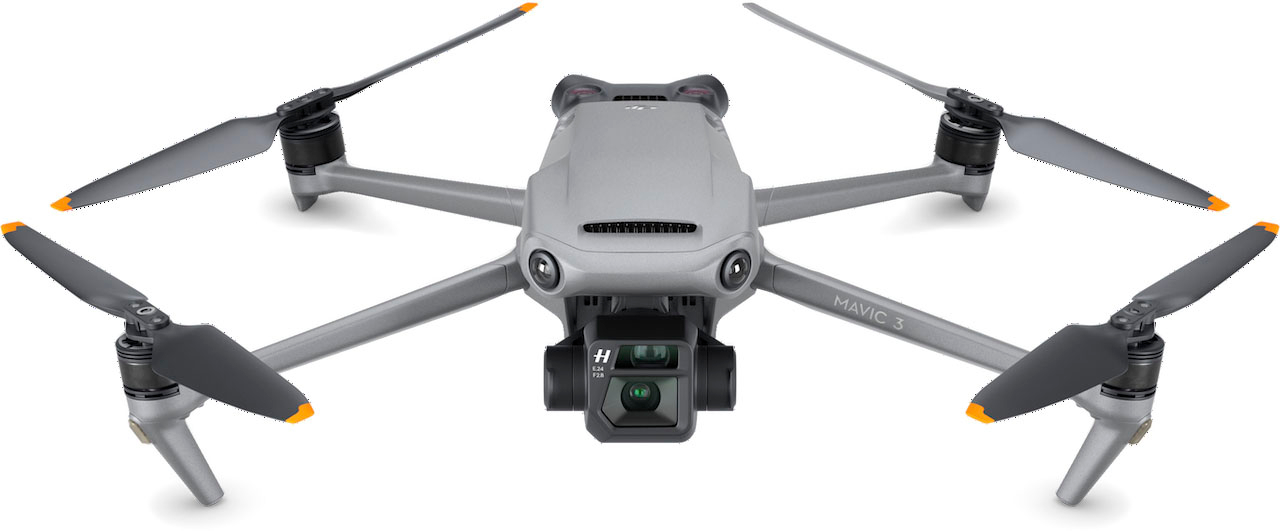
\includegraphics[width=0.7\textwidth]{proposal/quadcopter.jpg}
    \caption{DJI Mavic 3 Quadcopter}
    \label{fig:quadcopter_img}
\end{figure}

A quadcopter is a helicopter with four propellers arranged in a square formation. It can be controlled by rapidly changing the angular velocity of each rotor independently, such that a directional thrust and torque can be achieved about each rotor and likewise about the body of the drone. They have a wide variety of uses including aerial photography, search and rescue, agriculture, and surveillance \cite{luukkonen2011modelling}.

Although the structure is simple to construct and models are widely accessible on consumer markets, the dynamics and control systems required to make any use of the physical system are complex and nonlinear. In addition, quadcopters can be expensive and difficult to learn to control for a human operator. Thus, the setting is ideal for rigorous dynamical analysis, and a comprehensive numerical simulation of the quadrotor dynamics would be particularly helpful for someone that wishes to learn how to pilot one without running the risk of destroying it accidentally or otherwise damaging the drone or the surroundings.

In this work, I will derive the equations of motion of a quadcopter using the Euler-Lagrange equations, develop a simple PID controller to stabilize the drone horizontally, and present numerical simulations testing the validity of the dynamics and controller. The code and configurations used to generate these results are available at this \href{https://github.com/msc5/quadcopter}{public repository}.

\newpage
\section{Problem Setup}

\newcommand{\stau}{\boldsymbol{\tau}}

\subsection{Reference Frames}

Figure \ref{fig:frames} shows an inertial reference frame $\mathcal{I}$ as well as the body frame $\mathcal{B}$ of the quadcopter, which has its origin centered on the quadcopter's center of mass $G$ and principle axes aligned with the quadcopter's rotors. The positions of the rotors $\bar{r}_i$ are orthogonal to each other and have identical length $l$, and their orientations are fixed in the body frame, i.e., they cannot rotate independently of the drone structure. In the following derivations I will consider the drone structure as a rigid body with controllable point forces emitted upwards from the center of each rotor and moments which act about the center of each rotor. The effects of air resistance will be neglected.

\begin{figure}[H]
    \centering
    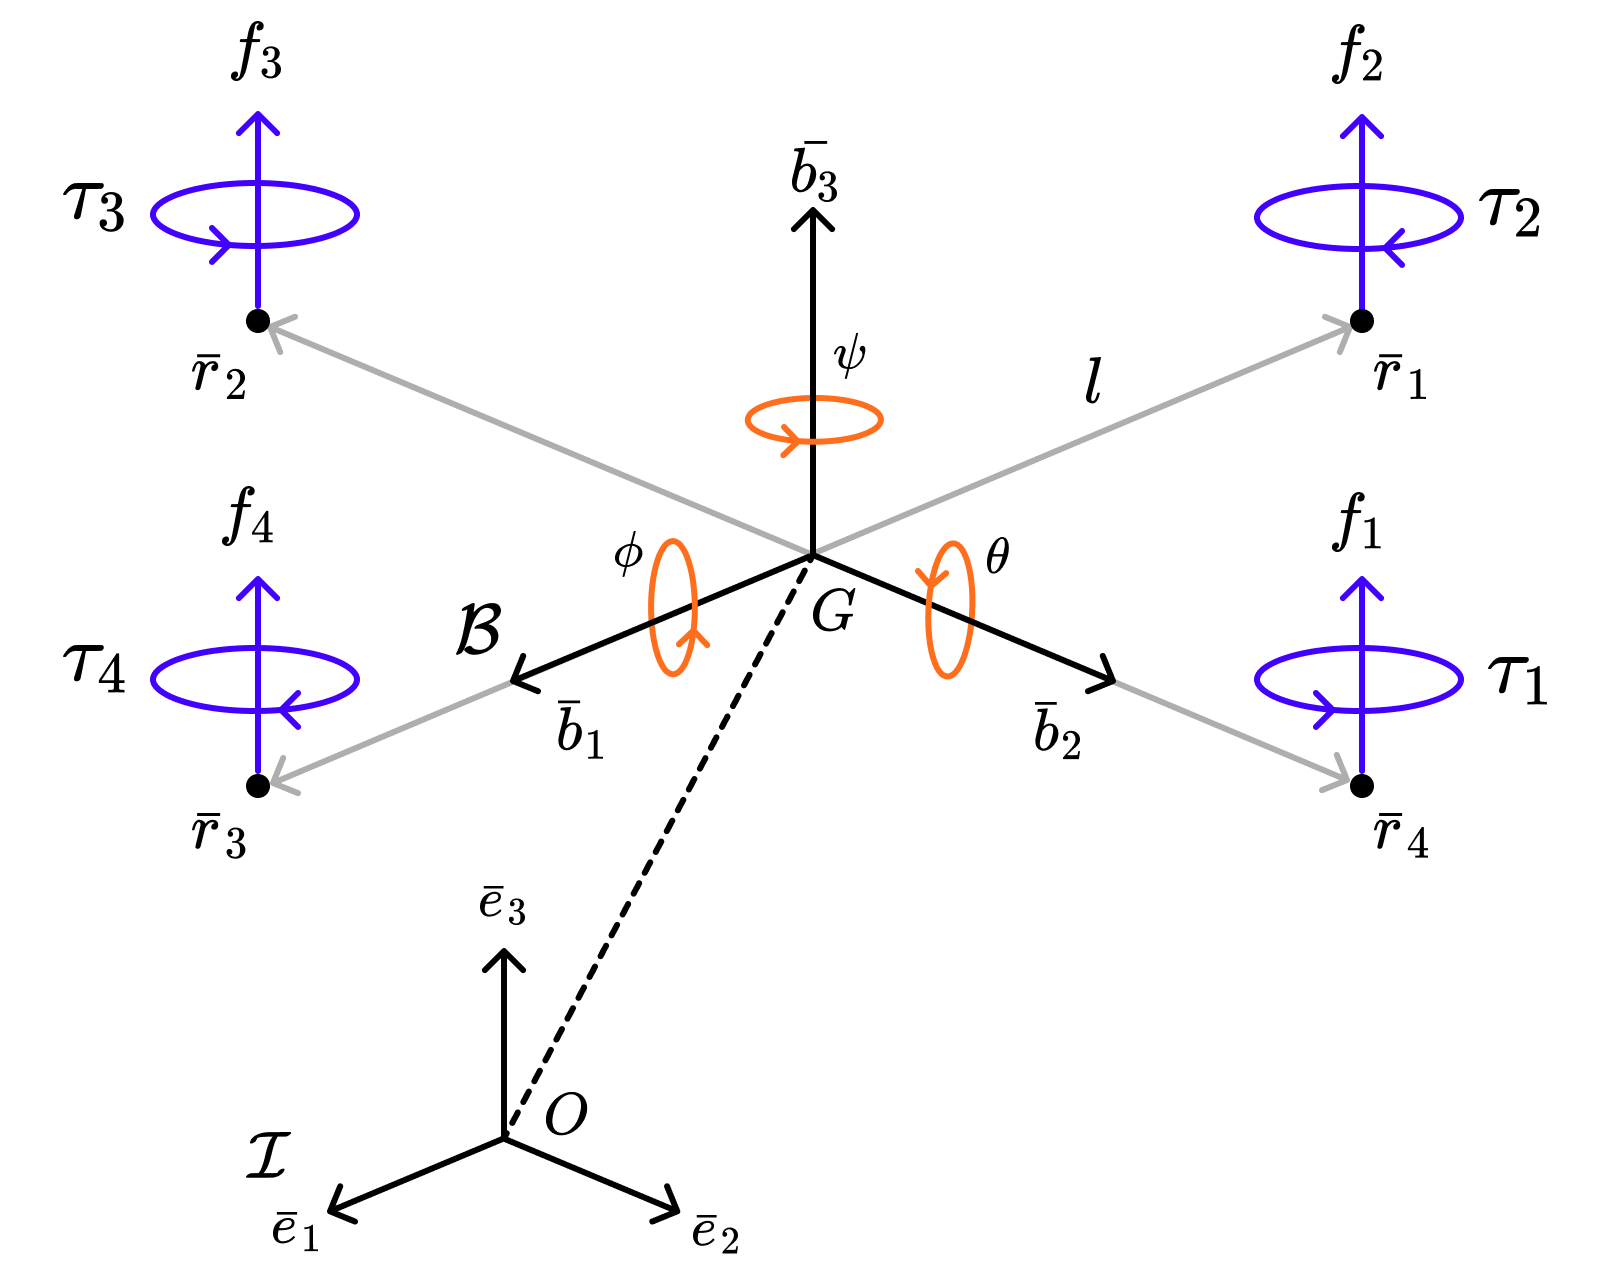
\includegraphics[width=0.7\textwidth]{figures/frames.png}
    \caption{Quadcopter frames, forces and moments}
    \label{fig:frames}
\end{figure}

With this setup laid out, the goal of this project is therefore to derive the equations of motion of the quadrotor using the Lagrangian formulation of dynamics and then to carry out numerical experiments using the results. From the figure, one can imagine that the evolution of the quadrotor state can easily become chaotic in flight, as it will be very easy for small changes in the roll or pitch of the body to produce oscillations or even invert the craft completely.

\subsection{Forces and Moments}

From Figure \ref{fig:frames} it is clear that the net force on the drone will be the sum of the 4 individual propeller thrusts acting upwards along the body frame vertical axes. Each propeller generates a thrust that is proportional to a constant $k$ multiplied by its angular velocity $\omega_i$ squared \cite{gibiansky2012andrew}. Thus:

\newcommand{\sF}{\boldsymbol{F}}
\newcommand{\sforce}{\boldsymbol{f}}

\begin{gather}
    f_i = k \omega_i^2
    , \quad
    \sF = k \begin{pmatrix} 0 & 0 & \sum_{i=1}^4 \omega_i^2 \end{pmatrix}^T
    , \quad
    \sforce = B \sF
\end{gather}

describes the force $\sF$ on the quadrotor center of mass in the body frame 
as well as the force $\sforce$ on the quadrotor center of mass in the inertial frame. The rotation matrix $B$ which maps vectors in the body frame to the inertial frame will be derived in the following section.

Furthermore, the moment produced by each rotor is proportional to a different constant $b$ multiplied by its angular velocity $\omega_i^2$ squared. Since each rotor is fixed and the moments produced by each blade are parallel, they can also be summed, i.e., $\stau_\psi = \sum_i \tau_i$. For $\stau_\theta$ and $\stau_\phi$, consider the forces produced by the pairs of rotors opposite each other about the origin. Also note, neighboring rotors spin in opposite directions. Thus:

\begin{gather}
    \stau = \begin{pmatrix} 
        l (f_1 - f_3) \\ l (f_2 - f_4) \\ \sum_{i=1}^4 \tau_i 
    \end{pmatrix}
    = \begin{pmatrix}
        kl (\omega_1^2 - \omega_3^2) \\ kl (\omega_2^2 - \omega_4^2) \\ 
        b (\omega_1^2 - \omega_2^2 + \omega_3^2 - \omega_4^2) 
    \end{pmatrix}
    \label{eqn:torque}
\end{gather}

\subsection{Rotation}

\newcommand{\lag}{\mathcal{L}}
\newcommand{\dd}[2]{\frac{d #1}{d #2}}
\newcommand{\pp}[2]{\frac{\partial #1}{\partial #2}}
\newcommand{\ddt}[1][]{\dd{#1}{t}}
\newcommand{\ppt}[1][]{\pp{#1}{t}}
\newcommand{\half}{\frac{1}{2}}
\newcommand{\W}{\Omega}
\DeclarePairedDelimiter\norm{\lVert}{\rVert}

\newcommand{\sq}{\boldsymbol{q}}
\newcommand{\sxi}{\boldsymbol{\xi}}
\newcommand{\seta}{\boldsymbol{\eta}}

Across several sources \cite{beard2008quadrotor, nakano2013quad, fresk2013full}, the most varied choice in deriving the dynamics of the quadcopter is the parametrization of rotation between the inertial frame $\mathcal{I}$ and body frame $\mathcal{B}$. The most straightforward approach, however, is the Euler-angle representation, which yields the rotation matrix $B$ through the composition of three rotations about a fixed principle axis.

Thus, the following generalized coordinates will be considered to parametrize the rotations:

\begin{gather}
    \seta = 
    \begin{pmatrix} \phi & \theta & \psi \end{pmatrix}^T
    , \quad 
    \dot{\seta} = 
    \begin{pmatrix}
        \dot{\phi} & \dot{\theta} & \dot{\psi}
    \end{pmatrix}^T
\end{gather}

Each component matrix of the Euler-angle representation along with the final representation itself are members of the special orthogonal group $SO(3)$. As we have seen in class, members of this group can be generated via matrix exponentials, i.e. (Using $c_\theta$ to represent $\cos{\theta}$ and $s_\theta$ to represent $\sin{\theta}$, etc.):

\renewcommand{\sin}[1]{\text{s}_{#1}}
\renewcommand{\cos}[1]{\text{c}_{#1}}

% \left\{ M \in \mathbb{R}^{3x3} \mid MM^T = \mathbb{I}_3, \det M = 1 \right\}$

\newcommand{\Rx}{
    \begin{pmatrix}
        1 & 0 & 0 \\
        0 & \cos{\phi} & -\sin{\phi} \\
        0 & \sin{\phi} & \cos{\phi} \\
    \end{pmatrix}}
\newcommand{\Ry}{
    \begin{pmatrix}
        \cos{\theta} & 0 & \sin{\theta} \\
        0 & 1 & 0 \\
        -\sin{\theta} & 0 & \cos{\theta} \\
    \end{pmatrix}}
\newcommand{\Rz}{
    \begin{pmatrix}
        \cos{\psi} & -\sin{\psi} & 0 \\
        \sin{\psi} & \cos{\psi} & 0 \\
        0 & 0 & 1 \\
    \end{pmatrix}}

\newcommand{\e}[1]{\exp \left( #1 \right)}

\begin{gather*}
    e^{\phi \hat{e}_1} = \Rx, \quad 
    e^{\theta \hat{e}_2} = \Ry, \quad 
    e^{\psi \hat{e}_3} = \Rz
\end{gather*}

There are numerous conventions of the rotation matrix, but in this case I will use the Tait-Bryan convention representing a sequence of yaw, pitch, and roll angles, which is the most common in the aerospace setting. Thus, the final representation of the rotation through $\psi$, $\theta$, and $\phi$ successively is given by the following:

\begin{align}
    B(\phi, \theta, \psi)
    & = 
    e^{\psi \hat{e}_3}
    e^{\theta \hat{e}_2}
    e^{\phi \hat{e}_1}
    \\
    & = 
    \begin{pmatrix}
        \cos{\psi} & -\sin{\psi} & 0 \\
        \sin{\psi} & \cos{\psi} & 0 \\
        0 & 0 & 1 \\
    \end{pmatrix}
    \begin{pmatrix}
        \cos{\theta} & 0 & \sin{\theta} \\
        0 & 1 & 0 \\
        -\sin{\theta} & 0 & \cos{\theta} \\
    \end{pmatrix}
    \begin{pmatrix}
        1 & 0 & 0 \\
        0 & \cos{\phi} & -\sin{\phi} \\
        0 & \sin{\phi} & \cos{\phi} \\
    \end{pmatrix} \\
     & = 
     \begin{pmatrix}
     \cos{\psi } \cos{\theta } & \sin{\phi } \sin{\theta } \cos{\psi } - \sin{\psi } \cos{\phi } & \sin{\phi } \sin{\psi } + \sin{\theta } \cos{\phi } \cos{\psi }\\\sin{\psi } \cos{\theta } & \sin{\phi } \sin{\psi } \sin{\theta } + \cos{\phi } \cos{\psi } & - \sin{\phi } \cos{\psi } + \sin{\psi } \sin{\theta } \cos{\phi }\\- \sin{\theta } & \sin{\phi } \cos{\theta } & \cos{\phi } \cos{\theta }
     \end{pmatrix}
     \label{eqn:B}
\end{align}

Equation \ref{eqn:B} provides a clear formulation of the rotation matrix $B$ as a function of $\seta$, however, it will also be useful to derive an expression for the angular velocity $\sOmega$ as a function of $\dot{\seta}$. To do this, we can consider each dimension of the angular velocity as each coordinate of $\dot{\seta}$ is transformed into the body-fixed frame $\mathcal{B}$.

\begin{align}
    \Omega_\phi 
    & = \begin{pmatrix} 1 \\ 0 \\ 0 \end{pmatrix} 
    \dot{\phi} \\
    \Omega_\theta = 
    \Rx \begin{pmatrix} 0 \\ 1 \\ 0 \end{pmatrix} \dot{\theta} 
    & = \begin{pmatrix} 0 \\ \cos{\phi} \\ \sin{\phi} \end{pmatrix} 
    \dot{\theta} \\
    \Omega_\psi = \Rx \Ry
    \begin{pmatrix} 0 \\ 0 \\ 1 \end{pmatrix}
    \dot{\psi} 
    & = 
    \begin{pmatrix} 
        \sin{\theta} \\ 
        -\cos{\theta} \sin{\phi} \\ 
        \cos{\theta} \cos{\phi}
    \end{pmatrix} 
    \dot{\psi}
\end{align}

\newcommand{\sOmega}{\boldsymbol{\Omega}}
\newcommand{\sW}{W_{\seta}}
\newcommand{\Wn}{
    \begin{pmatrix} 
        1 & 0 & \sin{\theta} \\
        0 & \cos{\phi} & -\cos{\theta} \sin{\phi} \\
        0 & \sin{\phi} & \cos{\theta} \cos{\phi}
    \end{pmatrix}}

Thus, the matrix $W_\seta$ can be derived, which transforms the time-derivative of the rotation state $\dot{\seta}$ into the angular velocity vector $\sOmega$:

\begin{align}
    \begin{pmatrix} \Omega_{\phi} \\ \Omega_{\theta} \\ \Omega_{\psi} \end{pmatrix}
    & = \underbrace{\Wn}_{\equiv \sW} 
    \begin{pmatrix} \dot{\phi} \\ \dot{\theta} \\ \dot{\psi} \end{pmatrix} \\
    \sOmega & = \sW \dot{\seta}
\end{align}

\subsection{State}

Along with the Euler-angle representation, I will consider the Cartesian coordinates of the center of mass of the drone as generalized coordinates to represent translations of the body frame:

\begin{align}
    \sxi =  \begin{pmatrix} x & y & z \end{pmatrix}^T
    , \quad
    \dot{\sxi} =  \begin{pmatrix} \dot{x} & \dot{y} & \dot{z} \end{pmatrix}^T
\end{align}

Thus, the following generalized coordinates together define a 6-degree-of-freedom dynamical system with the state $\sq$:

\begin{align}
    \sq = \begin{pmatrix} \sxi \\ \seta \end{pmatrix}
\end{align}

\newpage
\section{Dynamics}

\subsection{Lagrangian}

The Lagrangian $L$ is defined as:

\begin{align}
    L (\sq, \dot{\sq}) & = T - V 
\end{align}

This system is nearly identical to rigid body free rotation; however the Lagrangian has nonzero potential energy since the quadcopter is subject to gravity. As we have shown in class, the kinetic energy in this case is the same as in free rigid body rotation:

\begin{align}
    T & = 
    \underbrace{\half \sOmega^T I \sOmega}
    _{\substack{\text{Rotational kinetic} \\ \text{energy}}} + 
    \underbrace{\half m \dot{\sxi}^T \dot{\sxi}}
    _{\substack{\text{Translational kinetic} \\ \text{energy}}} \\ 
    & = 
    \half \dot{\seta}^T \underbrace{\sW^T I \sW}
    _{\equiv J (\seta)} \dot{\seta} +
    \half m \dot{\sxi}^T \dot{\sxi} \\
    & =
    \half \dot{\seta}^T J(\seta) \dot{\seta} +
    \half m \dot{\sxi}^T \dot{\sxi}
\end{align}

% Thus, the following are derivatives of $T$:

% \begin{align}
%     \pp{T}{\seta} 
%     & = 
%     \pp{}{\seta} \half \dot{\seta}^T \left( J (\seta) + m \right) \dot{\seta} \\
%     & = 
%     \half \dot{\seta}^T \left( \pp{}{\seta} J (\seta) \right) \dot{\seta} \\
%     & = 
%     \half \dot{\seta}^T \left( \pp{}{\seta} \left( \sW^T I \sW \right) \right) \dot{\seta}
% \end{align}

% \begin{align}
%     \pp{}{\seta} \left( \sW^T I \sW \right) & =
%     \pp{}{\seta} \left( \sW^T \right) I \sW +
%     \sW^T I \pp{}{\seta} \left( \sW \right)
% \end{align}

And the potential energy can be determined from these coordinates in the standard way using the gravitational potential:

\begin{align}
    V & = m g z = m g (\sxi \cdot \bar{e}_3)
\end{align}

Thus, the entire Lagrangian is given by:

\begin{align}
    L(\sq, \dot{\sq}) & = 
    \half \dot{\seta}^T J(\seta) \dot{\seta} +
    \half m \dot{\sxi}^T \dot{\sxi} -
    m g (\sxi \cdot \bar{e}_3)
\end{align}

\subsection{Translations}

Since the equation is linear, we can split the Lagrangian into a sum of two functions, i.e. $L(\sq, \dot{\sq}) = L(\seta, \dot{\seta}) + L(\sxi, \dot{\sxi})$ and consider them separately. First, the derivatives of $L(\sxi, \dot{\sxi})$, which are relatively straightforward to derive:

\begin{gather}
    \pp{L}{\sxi} = - mg \bar{e}_3 = 
    \begin{pmatrix} 0 & 0 & - mg \end{pmatrix}^T \\
    \pp{L}{\dot{\sxi}} = m \dot{\sxi} 
    , \quad 
    \ddt \pp{L}{\dot{\sxi}} = m \ddot{\sxi}
\end{gather}

These results lead to the following equation of motion for the translation dynamics of the quadcopter using the Euler-Lagrange Equation:

\newcommand{\sQ}{\boldsymbol{Q}}

\begin{align}
    \ddt \pp{L}{\dot{\sxi}} - \pp{L}{\sxi} & = \sforce \\
    m \ddot{\sxi} + m g \bar{e}_3 & = \sforce \\
    \ddot{\sxi} & = \frac{1}{m} \left( \sforce - mg \bar{e}_3 \right)
\end{align}

\subsection{Rotations}

The derivatives of $L(\seta, \dot{\seta})$, however, are more difficult to determine as they are higher-dimensional:

\begin{align}
    \pp{L}{\seta} & = 
    \half \pp{}{\seta} \left( \dot{\seta}^T J \right) \dot{\seta} 
    \label{eqn:dldeta} \\
    \pp{L}{\dot{\seta}}
    & = \half \pp{}{\dot{\seta}} \left( \dot{\seta}^T J \dot{\seta} \right) \nonumber
    = \half \pp{}{\dot{\seta}} \left( J \dot{\seta} \cdot \dot{\seta} \right) \\
    & = \half \pp{}{\dot{\seta}} \sum_i \left( J_{i *} \eta_i \right) \eta_i
    = \half \sum_i J_{i *} \pp{}{\dot{\seta}} \eta_i^2 \nonumber \\
    & = \sum_i J_{i *} \eta_i = J \dot{\seta} 
    \label{eqn:dldetad} \\
    \ddt \pp{L}{\dot{\seta}} & = \dot{J} \dot{\seta} + J \ddot{\seta}
    \label{eqn:ddtdldetad}
\end{align}

Equation \ref{eqn:dldeta} is the most complicated expression; it is a 3x3 Jacobian matrix, the derivative of a vector $\dot{\seta}^T J$ with respect to a vector $\seta$. What makes this expression difficult to compute, however, are the large amount of terms that come out of the derivative given that $J = \sW^T I \sW$. A full definition of this variable is given in the appendix section \ref{app:coriolis}. Equation \ref{eqn:dldetad}, however, is more like a normal derivative; the product rule can be used to split the derivative into a sum of dot products and then computed using a summation, eventually leading to the definition of matrix multiplication which yields $J \dot{\seta}$.

The equation of rotational motion can also be determined using the Euler-Lagrange Equation:

\begin{align}
    \ddt \pp{L}{\dot{\seta}} - \pp{L}{\seta} & = \stau \\
    \dot{J} \dot{\seta} + J \ddot{\seta} + 
    \half \pp{}{\dot{\seta}} \left( \dot{\seta}^T J \right) \dot{\seta}
    & = \stau \\
    J \ddot{\seta} + \underbrace{
    \left( \dot{J} +\half \pp{}{\dot{\seta}} \left( \dot{\seta}^T J \right) \right)}
    _{\equiv C(\seta, \dot{\seta})}
    \dot{\seta}
    & = \stau \\
    J \ddot{\seta} + C(\seta, \dot{\seta}) \dot{\seta}
    & = \stau \\
    \ddot{\seta} & = 
    J^{-1} \left( \stau - C(\seta, \dot{\seta}) \dot{\seta} \right) \\
\end{align}

Here, the Jacobian matrix previously discussed as well as the time-derivative of $J$ are combined into the Coriolis matrix $C(\seta, \dot{\seta})$. The complete equations of motion of the quadrotor are thereby given by the following system:

\begin{equation}
    \begin{cases}
        \ddot{\sxi} & = \frac{1}{m} \left( \sforce - mg \bar{e}_3 \right) \\
        \ddot{\seta} & = 
        J^{-1} \left( \stau - C(\seta, \dot{\seta}) \dot{\seta} \right)
    \end{cases}
\end{equation}

% Lagrange's Equation is given by:
% 
% \begin{align}
%     \ddt \dd{L}{\dot{\sq}} - \dd{L}{\sq} & = \boldsymbol{Q} \\
%     \dd{L}{\sq} & = 
% \end{align}

\newpage
\section{Controls}
\label{sec:controls}

\newcommand{\su}{\boldsymbol{u}}
\newcommand{\se}{\boldsymbol{e}}

In order to better test the simulation of the dynamics, it will be useful to first derive a simple PID controller to stabilize the drone horizontally, i.e., $\seta, \dot{\seta} \rightarrow 0$. To do this, I will consider a controller $\su$ which takes $\dot{\seta}$ as an input and outputs the angular velocity of each propeller $\omega_i$. The controller is defined as follows \cite{gibiansky2012andrew}:

\begin{align}
    \se & = \seta^c - \seta = \seta \\
    \su & = k_p \se + k_i \int_0^t \se dt + k_d \ddt \se \\
    & = k_p \seta + k_i \int_0^t \seta dt + k_d \dot{\seta}
\end{align}

The controller generates a torque about the center of mass of the quadcopter, which is described in Equation \ref{eqn:torque} (Let $\gamma_i = \omega_i^2$). If we ignore the Coriolis matrix (which is not an unreasonable approximation; it is composed of nearly all higher-order terms) then we have the following equation for the controller:

\begin{align}
    \begin{pmatrix}
        kl (\gamma_1 - \gamma_3) \\ kl (\gamma_2 - \gamma_4) \\ 
        b (\gamma_1 - \gamma_2 + \gamma_3 - \gamma_4) 
    \end{pmatrix} =
    J \su
\end{align}

\newcommand{\sj}{\boldsymbol{j}}

However, this is a system of 4 unknowns and only 3 equations. If we further constrain the sum of generated forces to keep the quadrotor hovering, i.e., $\sforce_3 = mg \bar{e}_3$, then we have an additional constraint. Note, in order to generate this force in the inertial frame, the drone must generate a force $T = \frac{mg}{\cos{\theta} \cos{\phi}}$ in the body frame. This leads to the following system of equations (Let $J \su = \sj$, $\sj_i = j_i$):

\begin{align}
    \begin{pmatrix}
        kl (\gamma_1 - \gamma_3) \\ kl (\gamma_2 - \gamma_4) \\ 
        b (\gamma_1 - \gamma_2 + \gamma_3 - \gamma_4) \\
        k (\gamma_1 + \gamma_2 + \gamma_3 + \gamma_4)
    \end{pmatrix} =
    \begin{pmatrix} j_1 \\ j_2 \\ j_3 \\ T \end{pmatrix}
\end{align}

This system has the following solution:

\begin{align}
    \begin{pmatrix} \gamma_1 \\ \gamma_2 \\ \gamma_3 \\ \gamma_4 \end{pmatrix} =
    \frac{T}{4k} + 
    \frac{1}{2 k l}
    \begin{pmatrix} -j_1 \\ -j_2 \\ j_2 \\ j_2 \end{pmatrix} +
    \frac{1}{4 b}
    \begin{pmatrix} -j_3 \\ j_3 \\ -j_3 \\ j_3 \end{pmatrix}
\end{align}

\newpage
\section{Simulations}

\subsection{Pure Dynamics}

\newcommand{\traj}[3]{
    \begin{figure}[H]
        \centering
        \begin{minipage}{0.65\textwidth}
            \centering
            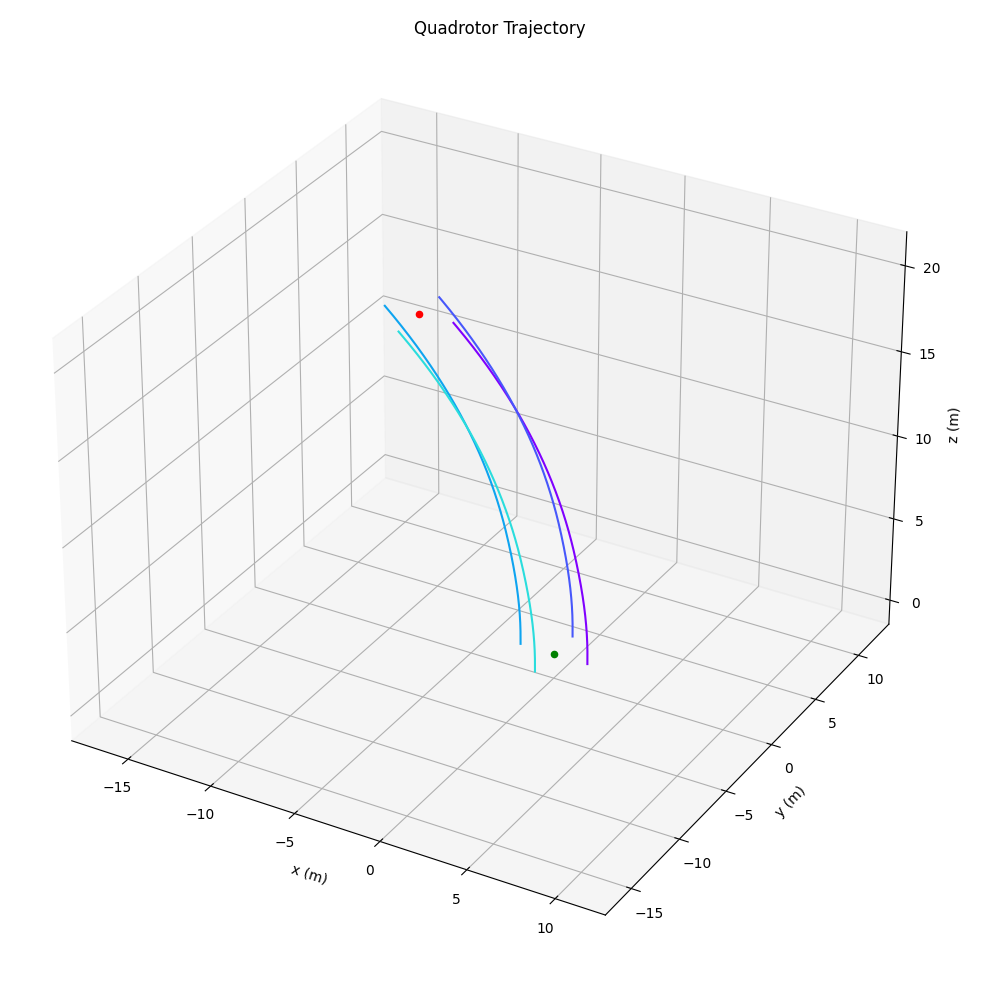
\includegraphics[width=1\textwidth]{figures/#1/traj3d.png}
        \end{minipage}
        \begin{minipage}{0.85\textwidth}
            \centering
            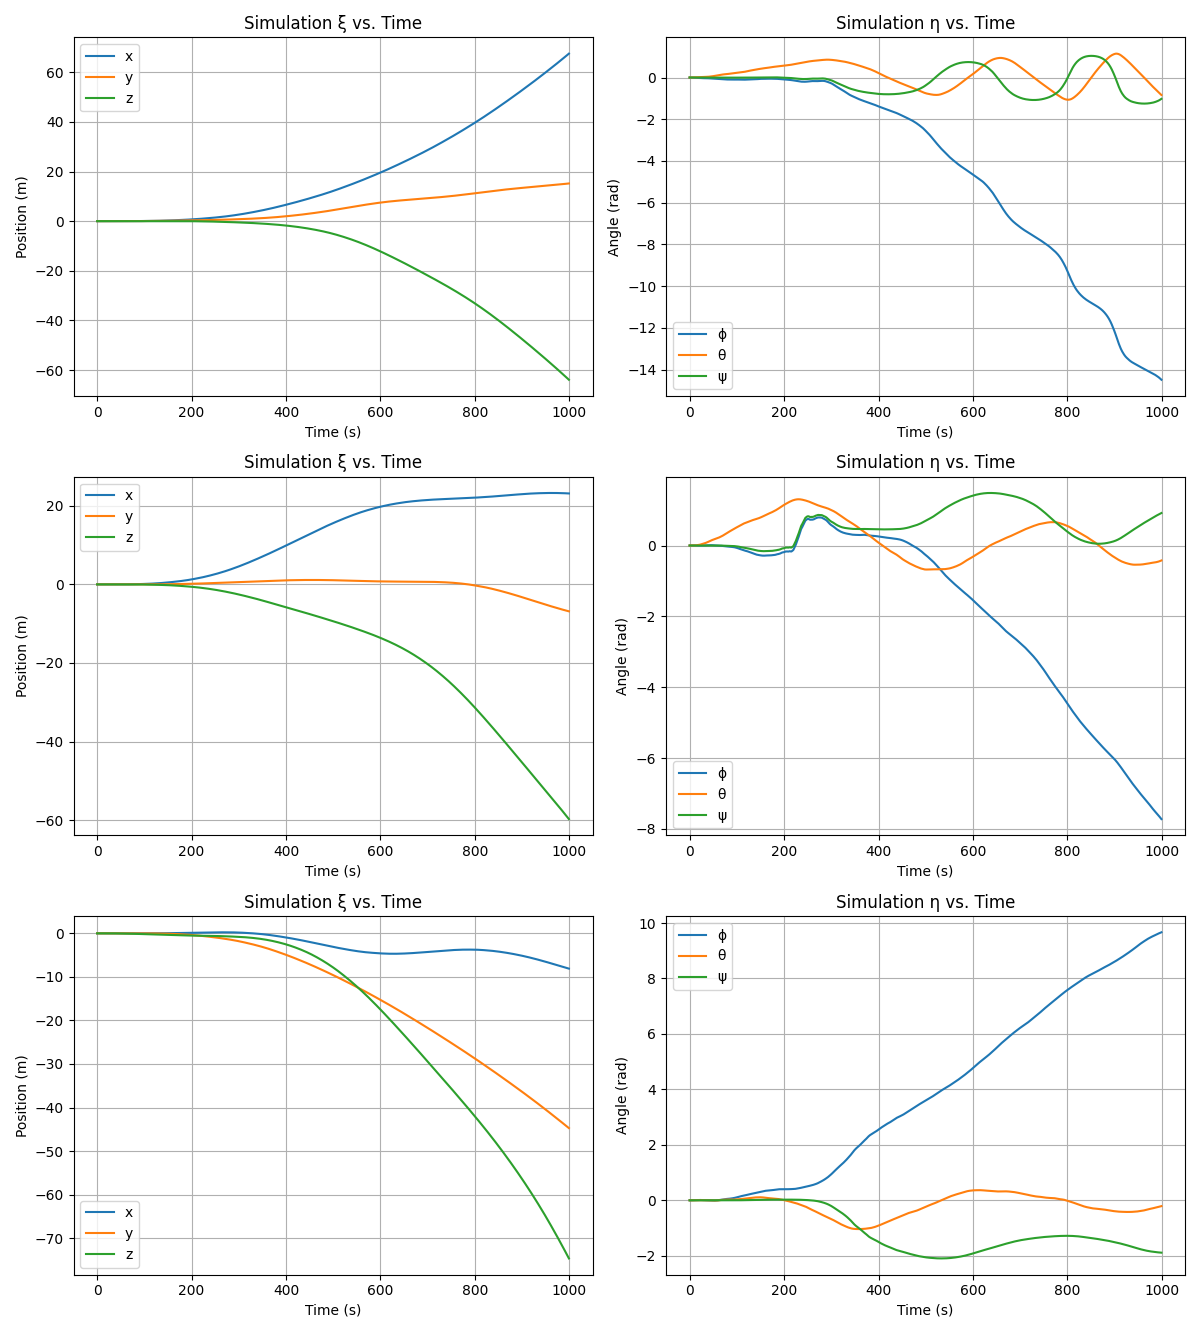
\includegraphics[width=1\textwidth]{figures/#1/traj2d.png}
        \end{minipage}
        \caption{#2}
        \label{#3}
    \end{figure}}

In the absence of a physical drone to carry out experiments, I will conduct a series of simulated experiments and test assumptions made about the dynamics of the system in order to validate the equations of motion. These simple results are more of a sanity check than anything, to ensure that the simplest quadcopter maneuvers are accurately captured by the dynamics. Each trajectory is represented by four ``traces'' showing the path of each rotor, which starts at a blue color and gradually becomes pink as time progresses.

The first assumption is that applying a net upward force slightly greater than the weight of the quadcopter split across each rotor (with zero torque) should lead to a straight takeoff. Figure \ref{fig:takeoff_straight} supports this hypothesis, showing an increase in the z coordinate that grows steeper over time.

\traj{takeoff-straight}{Straight Takeoff}{fig:takeoff_straight}

In the next experiment, I will simulate a similar takeoff condition, except with an initial angular velocity imposed on the quadcopter, such that the trajectory immediately becomes unstable. These conditions test the limits of the numerical integration technique, however, with enough precision it is possible to determine the flight path of the drone and its wild oscillations in this state. The results of this experiment also show the instability that nearly all modes of quadrotor flight exhibit. Once tumbling in such a manner, it is difficult even for a well-tuned controller to stabilize the drone.

\traj{tumble}{Tumble}{fig:tumble}

Again, these results are not meant to provide a useful example of the quadrotor dynamics, but rather to display empirical results of the derived equations of motion and to verify that simple expectations about the flight of a quadcopter can be reproduced in the simulation. In the next section, I will present experiments carried out with an actually useful controller.

\subsection{Simulated Control}

One of the simplest tests to carry out using the controller described in Section \ref{sec:controls} is a step response, in which the quadcopter starts out with a nonzero initial angular position and velocity and uses the controller to drive this error to zero. In this experiment, the initial angular velocity used was twice the amount of the angular velocity used in the ``Tumble'' experiment (Figure \ref{fig:tumble}).

\traj{step}{Step Response}{fig:step}

In this response, note that the quadcopter was able to also stay steady in the z-axis; this is because the controller is designed to always produce an upwards thrust equal to the quadcopter's weight, regardless of its orientation. Within 5 seconds of this simulation, the quadcopter is able to drive both its angular velocity and position to zero as hypothesized. Despite the efforts of the controller, however, there is still some ``drift'' during the maneuver. This is to be expected, since the controller does not depend on the x or y position and only depends on the rotation.

\traj{recovery}{Takeoff Recovery}{fig:recovery}

For the final test, I simulate a ``faulty takeoff,'' (or simply, a delayed step response) in which two neighboring propellers are jammed and produce less thrust than the opposite two, leading to a tilt and imminent tumble. A quarter of the way through the simulation, however, the stabilizing controller turns on and is able to quickly correct the misalignment.

\newpage
\section{Discussion}

In this project I have shown how to derive the equations of motion of a quadcopter using the Lagrangian formulation of dynamics and verified the result using numerical methods. Additionally, I have implemented a simple PID control system to stabilize the drone horizontally and likewise verified its effectiveness in simulations. While the dynamics of a quadcopter can be derived in varying levels of complexity, this work shows that even a simple approach using the Euler-Lagrange equations can yield substantial results when combined with numerical simulation, and although the derived equations are simple enough, they describe an extremely detailed evolution of the physical system that can be used for many purposes.

Some directions for future work involve more complex methods of representing the rotations of a rigid body in 3D, for example, quaternions, which don't suffer from gimbal lock, and of course more effective controllers which can be implemented using these parametrizations \cite{fresk2013full}. Also, there are countless specific applications for quadcopters which can be studied more directly from the perspective of the dynamics, for example in FPV drone racing where it is necessary to maximize the speed of the drone to gain a competitive edge, or in surveillance where sound generated by the rotors could be a main concern. 

Another course of interest could be to focus on the numerical simulation itself, as numerical methods are key to realizing the power of any dynamics derivation, and there are more advanced integration methods (for example, Runge-Kutta) than the naive Euler integration used in this project, which could potentially improve the realism of the simulated results as well as prevent divergence when functions are not smooth. 

\newpage
\bibliography{main}

\newpage
\section{Appendix}

\subsection{Coriolis Matrix}
\label{app:coriolis}

The entire Coriolis Matrix $C(\seta, \dot{\seta})$ is given by the following expression \cite{nakano2013quad}:

\begin{figure}[H]
    \centering
    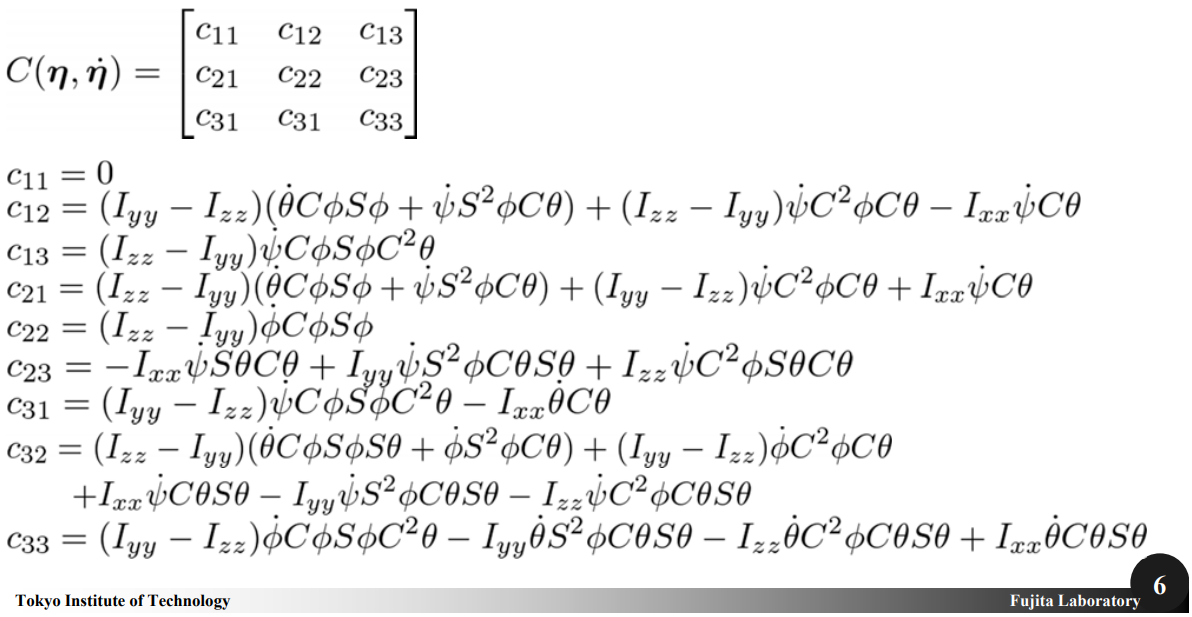
\includegraphics[width=1\textwidth]{figures/cmatrix.png}
    \caption{Coriolis Matrix}
    \label{fig:coriolis}
\end{figure}

\end{document}
